\subsection{Medium-Scale Anchor and Existing-Trace Diagnosis}
\label{sec:medium_evidence}

\smallTitle{Separate evaluation scope}
To examine the primary findings beyond four routes, a separate campaign evaluates 15 nodes and ten candidate routes under Default/fixed allocation: 90 qubits, nine per route, and 55 feasible three-component allocation actions per route. Oracle, GNeuralUCB (G), EXPNeuralUCB (EXP), CPursuitNeuralUCB (CP), and iCPursuitNeuralUCB (iCP) each run under all five threat settings in three blocks of 6,000 frames. All 75 cells completed without technical retries or performance-driven reruns. The accepted traces comprise 450,000 decision frames and 1.8 million phase records; phase records are not independent replications. Replay is fixed to $T_b$ anchoring, base horizon 6,000, scale two, and capacity 12,000. This is one medium anchor, not a controlled scale curve or an allocator/replay sweep.

\smallTitle{Outcome and comparator}
For this campaign, payoff is the recorded continuous selected base payoff multiplied by route availability, not a count of successful quantum deliveries. In block $b$, threat $h$, and window $W$, efficiency is
\[
E_{b,h,W}=100\frac{\sum_{t\in W}u^{\mathrm{policy}}_{b,h,t}}
{\sum_{t\in W}u^{\mathrm{Oracle}}_{b,h,t}}.
\]
We average the three block ratios equally, not by pooling payoff sums. Oracle knows the catalog payoffs and current availability and maximizes that frame's available payoff. Under reactive threats, policies induce different availability histories; the Oracle gap is therefore a privileged descriptive comparison, not a causal learning deficit. Diagnostics use prespecified early (1--2,000), middle (2,001--4,000), and late (4,001--6,000) windows and twelve disjoint 500-frame bins. Three-block dispersion is descriptive, not inferential significance.

\begin{table*}[t]
\centering\scriptsize
\setlength{\tabcolsep}{2pt}
\caption{Medium-campaign full-horizon efficiency (\%), equal-block mean $\pm$ sample SD, $n=3$. G, EXP, CP, and iCP denote the four learned neural policies defined in the text.}
\label{tab:medium_efficiency}
\begin{tabular}{lrrrr}
\toprule
Threat & G & EXP & CP & iCP\\
\midrule
Baseline & $3.814\pm1.230$ & $3.124\pm1.124$ & $3.867\pm1.195$ & $3.276\pm1.938$\\
Stochastic & $3.611\pm1.201$ & $2.852\pm1.183$ & $3.623\pm1.136$ & $2.948\pm1.906$\\
Markov & $1.742\pm0.584$ & $1.407\pm0.698$ & $2.054\pm1.140$ & $1.112\pm0.546$\\
Adaptive & $2.769\pm1.001$ & $2.282\pm1.111$ & $3.095\pm1.289$ & $2.277\pm1.488$\\
OnlineAdaptive & $0.056\pm0.060$ & $0.066\pm0.010$ & $0.007\pm0.012$ & $0.000\pm0.000$\\
\bottomrule
\end{tabular}
\end{table*}

\smallTitle{Compression and conditional ordering}
\Cref{tab:medium_efficiency} shows learned means of 1.1122--3.8674\% outside OnlineAdaptive and 0--0.0662\% within it. CP leads four full-horizon threat means but only one of three blocks within each; EXP leads the OnlineAdaptive full mean, with only 15 positive-payoff frames over 18,000 decisions. Early-to-late mean leaders change from CP to G in Baseline/Stochastic, EXP to CP in Markov, and EXP to iCP in Adaptive. In late OnlineAdaptive, EXP leads mean absolute payoff but G leads equal-block normalized efficiency. No stable superiority or statistical equivalence follows from the clustered means.

\smallTitle{Observed behavior, not an isolated cause}
A structural-zero selection has catalog base payoff exactly zero; a realized-zero selection has continuous payoff zero. Baseline availability is complete, yet learned policies select structural-zero actions on 87.7167--90.2611\% of frames on average. Every learned cell visits all ten routes, while Baseline cells visit only 133--185 of 550 route/action pairs. Thus the sparse exposure is within-route, not missing route coverage. These measurements identify where payoff is lost arithmetically, but do not isolate why actions are selected or require exhaustive exploration by a contextual learner. Late payoff exceeds early payoff in 47 of 48 non-OnlineAdaptive learned cells. Final-window slopes have mixed signs: behavioral change is observed, convergence is not established, and a longer horizon is not a demonstrated remedy.

\begin{figure*}[t]
\centering
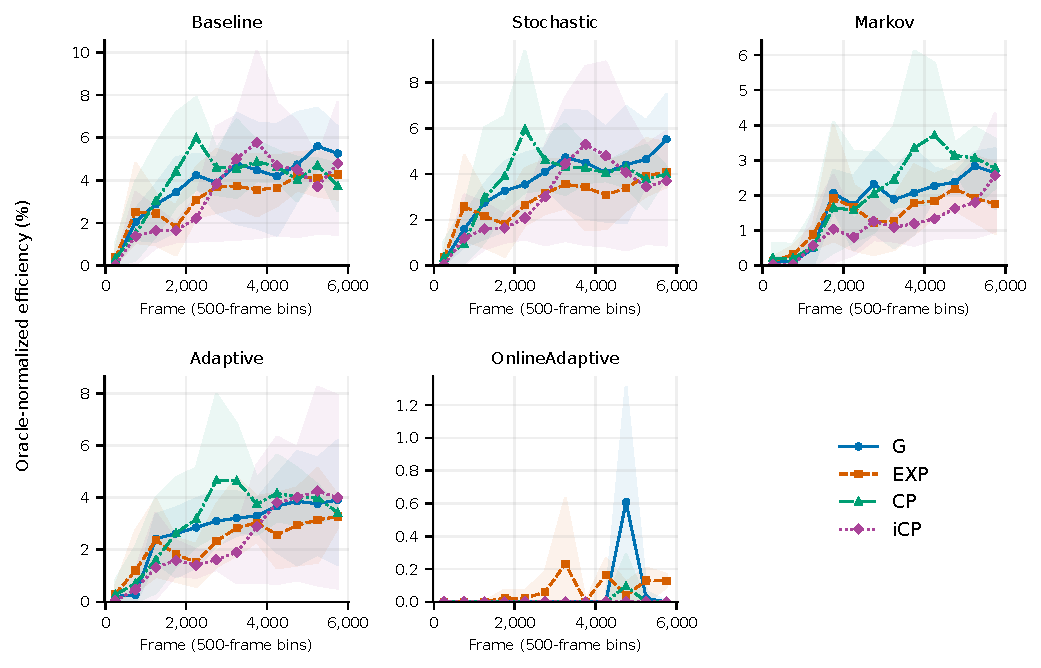
\includegraphics[width=\textwidth]{figures/icnp/medium_efficiency_trajectory.pdf}
\caption{Accepted medium-campaign trajectories in disjoint 500-frame bins. Lines are equal-block means and shading is the three-block range, not a confidence interval. Axes differ across threats. Reactive-threat ratios compare policy-conditioned histories; visual flattening is not evidence of convergence.}
\label{fig:medium_trajectory}
\end{figure*}

\smallTitle{Feedback and severe availability stress}
G, EXP, and CP each record zero positive sampled Bernoulli route-feedback draws over 90,000 decisions, but their within-route learners still receive continuous allocation feedback. Summed recorded Bernoulli draw probabilities are only 0.490, 0.407, and 0.518, respectively; zero positive draws alone do not establish a defective sampler. iCP uses a distinct continuous route-feedback channel. Under OnlineAdaptive, global availability is 8,343/180,000 route-frames (4.635\%) per model, and all routes are unavailable in 12,868/18,000 frames (71.4889\%). Selected-route availability is 2.1556\% for G/CP/iCP, 4.5\% for EXP, and 28.5111\% for Oracle. Among available selections, structural zeros still account for 385/388 (G), 795/810 (EXP), 387/388 (CP), and 388/388 (iCP). Availability scarcity alone therefore does not account for all zero payoff. Equal global availability totals also do not imply equal reactive masks.

The accepted diagnosis establishes these medium-setting observations, not a cause of the historical 100-node result. Action exposure, horizon, feedback scale, physics, and reactive history remain coupled; neither node count alone nor any one diagnostic is an identified explanation of cross-testbed compression.
